\documentclass[11pt]{article}

\usepackage[utf8]{inputenc}
\usepackage[T1]{fontenc}
\usepackage{amsmath,amssymb,amsfonts}
\usepackage{graphicx}
\usepackage[margin=1in]{geometry}
\usepackage[numbers,sort&compress]{natbib}
\usepackage{booktabs}
\usepackage{siunitx}
\usepackage{hyperref}
\usepackage{longtable}
\usepackage{array}
\usepackage{float}
\usepackage{xcolor}
\graphicspath{{../figures/}}

\title{\textbf{Realistic Universal Hybrid Control in the Dispersive cQED Regime:\\
What Survives Beyond the Ideal Primitive Gate Set?}}
\author{cQED Autonomous Research Platform \\ Shyam Shankar Quantum Circuits Group}
\date{\today}

\begin{document}

\maketitle

\begin{abstract}
The ideal universal-control claim for a dispersive transmon--cavity system is usually stated in terms of three primitives: selective qubit rotations, cavity displacements, and unconditional qubit rotations. The present study asks whether that claim survives the realistic dispersive Hamiltonian once the leading dispersive shift $\chi$, higher-order correction $\chi'$, cavity self-Kerr, and finite-duration phase accumulation are enforced. Rather than rerunning the entire repository, we combine a first-principles control-timescale analysis with the validated machine-readable results of the displacement-focused, waveform-level, literature-informed selective-pulse, strict-SQR, relaxed-CPSQR, arbitrary-conditional-control, and runtime hybrid-unitary studies already completed in the same simulation environment.

The central result is negative in its literal form but positive in a weaker, more physical form. The strict ideal primitive library does \emph{not} survive unchanged. Unconditional displacement is only reliable for very short, explicitly branch-compensated pulses: the best simple two-tone protocol reaches mean broad-state fidelity $0.9857$ at $|\chi|T/2\pi=0.057$. Vacuum-calibrated qubit rotations are not truly unconditional once photons populate the cavity; at \SI{40}{ns} the vacuum $X_\pi$ fidelity is $0.99984$, but the same pulse becomes strongly number dependent and the reported fidelity falls to about $0.483$ by the $n=5$ manifold. By contrast, relaxed phase-aware selective control is robust: the best noisy conditional-phase selective qubit rotation reaches average relaxed fidelity $0.9903$ at $|\chi|T/2\pi=1.0$, and segmented relaxed control reaches essentially unit relaxed joint-process fidelity on hard arbitrary-target slices. Strict full-joint ideal selective qubit rotation remains possible only on easier low-dimensional cases, with the strongest direct multitone example reaching joint process fidelity $0.9988$ at $|\chi|T/2\pi=5.0$, while the harder $\chi+\chi'$ cases and arbitrary-target classes fail to support a general positive claim. At the full-sequence level, even the best replay-backed hybrid-unitary candidate in the repository still requires GRAPE-derived local surrogates and falls to noisy average probe fidelity $0.614$ at total duration \SI{4.432}{\micro s}.

The defensible conclusion is therefore precise. The abstract ideal primitive gate set does not survive literally. What survives is a weaker, phase-aware constructive library consisting of short branch-compensated displacement, short spectator-limited qubit pulses, relaxed selective qubit control, and an explicit gauge-cleanup layer such as SNAP or virtual-$Z$ correction. That library is scientifically credible and practically useful on low-dimensional logical windows, but a fully validated non-GRAPE universal-control stack is not yet demonstrated.
\end{abstract}

\section{Introduction}

Universal control of a hybrid transmon--cavity system is one of the central conceptual promises of dispersive circuit QED. In the ideal abstraction, number selectivity generated by the dispersive shift can be combined with cavity translations and qubit rotations to synthesize arbitrary joint operations on the qubit plus oscillator \cite{koch2007transmon,blais2021circuit,krastanov2015universal}. The attraction of that picture is not only formal controllability. It suggests a structured and experimentally interpretable route to bosonic quantum information processing, avoiding the need to treat every useful operation as an opaque optimal-control waveform.

The difficulty is that the same dispersive Hamiltonian that creates number selectivity also destabilizes the ideal primitive picture. Once photons occupy the cavity, qubit transitions become manifold dependent through $\chi$ and $\chi'$, cavity displacements become branch dependent, and all finite-duration pulses accumulate conditional dynamical phase. In practice the natural question is therefore not whether some numerical waveform can solve some finite-dimensional control problem, but whether the \emph{ideal primitive library itself} survives as a realistic and physically deployable description.

This study addresses that question directly. The main contribution is a first-principles synthesis of the validated evidence already produced in this repository under a common simulation stack. The result is more informative than a single new optimization pass because the existing studies isolate different pieces of the problem:
\begin{itemize}
\item the displacement-focused study identifies when cavity translations cease to be unconditional;
\item the waveform-level study quantifies spectator failure of vacuum-calibrated qubit rotations;
\item the literature-informed selective-pulse study identifies the best practical relaxed selective-rotation and SNAP pulse families under noise;
\item the strict-SQR and arbitrary-conditional-control studies determine when full-joint selective control really survives, and when it survives only after an explicit gauge relaxation;
\item the runtime hybrid-unitary study shows how far current constructive architectures remain from a deployment-ready universal stack once realistic replay is enforced.
\end{itemize}

The core scientific question is then sharp: does the ideal universal-control claim survive realistic dispersive dynamics, or must it be replaced by a weaker phase-aware claim?

\section{System and First-Principles Constraints}
\label{sec:system}

\subsection{Hamiltonian and Control Model}

The common effective Hamiltonian across the inherited studies is
\begin{equation}
\frac{H}{\hbar} =
\omega_c a^\dagger a
 +
\omega_q b^\dagger b
 +
\frac{\alpha}{2} b^{\dagger 2} b^2
 +
\chi\, a^\dagger a\, b^\dagger b
 +
\chi' \, a^\dagger a (a^\dagger a - 1)\, b^\dagger b
 +
\frac{K}{2} a^\dagger a (a^\dagger a - 1)
 +
H_d^{(q)}(t)
 +
H_d^{(c)}(t),
\label{eq:hamiltonian}
\end{equation}
where $a$ acts on the cavity mode, $b$ acts on the transmon, $\alpha$ is the transmon anharmonicity, $\chi$ is the leading dispersive shift, $\chi'$ is the higher-order dispersive correction, and $K$ is the cavity self-Kerr. The nominal device point used throughout the repository is
\begin{align}
\omega_q/2\pi &= \SI{6.150}{GHz}, &
\omega_c/2\pi &= \SI{5.241}{GHz}, \nonumber\\
\alpha/2\pi &= \SI{-255}{MHz}, &
\chi/2\pi &= \SI{-2.84}{MHz}, \nonumber\\
\chi'/2\pi &= \SI{-21}{kHz}, &
K/2\pi &= \SI{-28}{kHz}.
\label{eq:device}
\end{align}

Two finite-duration phase channels dominate the control logic.

\paragraph{Selective qubit control.}
At cavity photon number $n$, the qubit detuning relative to the vacuum branch is
\begin{equation}
\delta_q(n)/2\pi \approx n \chi/2\pi + n(n-1)\chi'/2\pi .
\label{eq:qubit_detuning}
\end{equation}
Spectral selectivity therefore benefits from larger $|\chi|T/2\pi$, but spectator-indifferent qubit control requires the same quantity to remain small over the occupied manifold window.

\paragraph{Cavity translation.}
For an unconditional displacement, the cavity drive must produce nearly the same coherent translation in the qubit-ground and qubit-excited branches. In the minimal dispersive picture the branch mismatch is controlled by $|\chi|T/2\pi$, while self-Kerr contributes an additional phase shear that scales as $|K| \bar{n} T / 2\pi$ on a coherent-state envelope. A long pulse is therefore simultaneously easier to spectrally resolve and harder to keep unconditional.

\subsection{The Fundamental Timing Conflict}

The inherited repository evidence compresses into one clean principle: the realistic primitive library is constrained by incompatible timing requirements. For the nominal device point,
\begin{equation}
\frac{1}{|\chi|/2\pi} \approx \SI{352}{ns}.
\label{eq:chi_timescale}
\end{equation}
The selective protocols that work best numerically occupy the regime
\begin{equation}
|\chi|T/2\pi \sim 1 \text{ to } 5,
\label{eq:selective_regime}
\end{equation}
whereas the operations that remain close to unconditional occupy the regime
\begin{equation}
|\chi|T/2\pi \ll 1.
\label{eq:unconditional_regime}
\end{equation}
This is not a software artifact. It is the direct control consequence of Eqs.~\eqref{eq:qubit_detuning}--\eqref{eq:unconditional_regime}.

Figure~\ref{fig:timescale} summarizes the repository's practical operating points on the common axis $|\chi|T/2\pi$. The central physical message is immediate: unconditionality and selectivity are not different names for the same pulse regime. They occupy different regions of control space and therefore require different pulse families.

\begin{figure}[H]
\centering
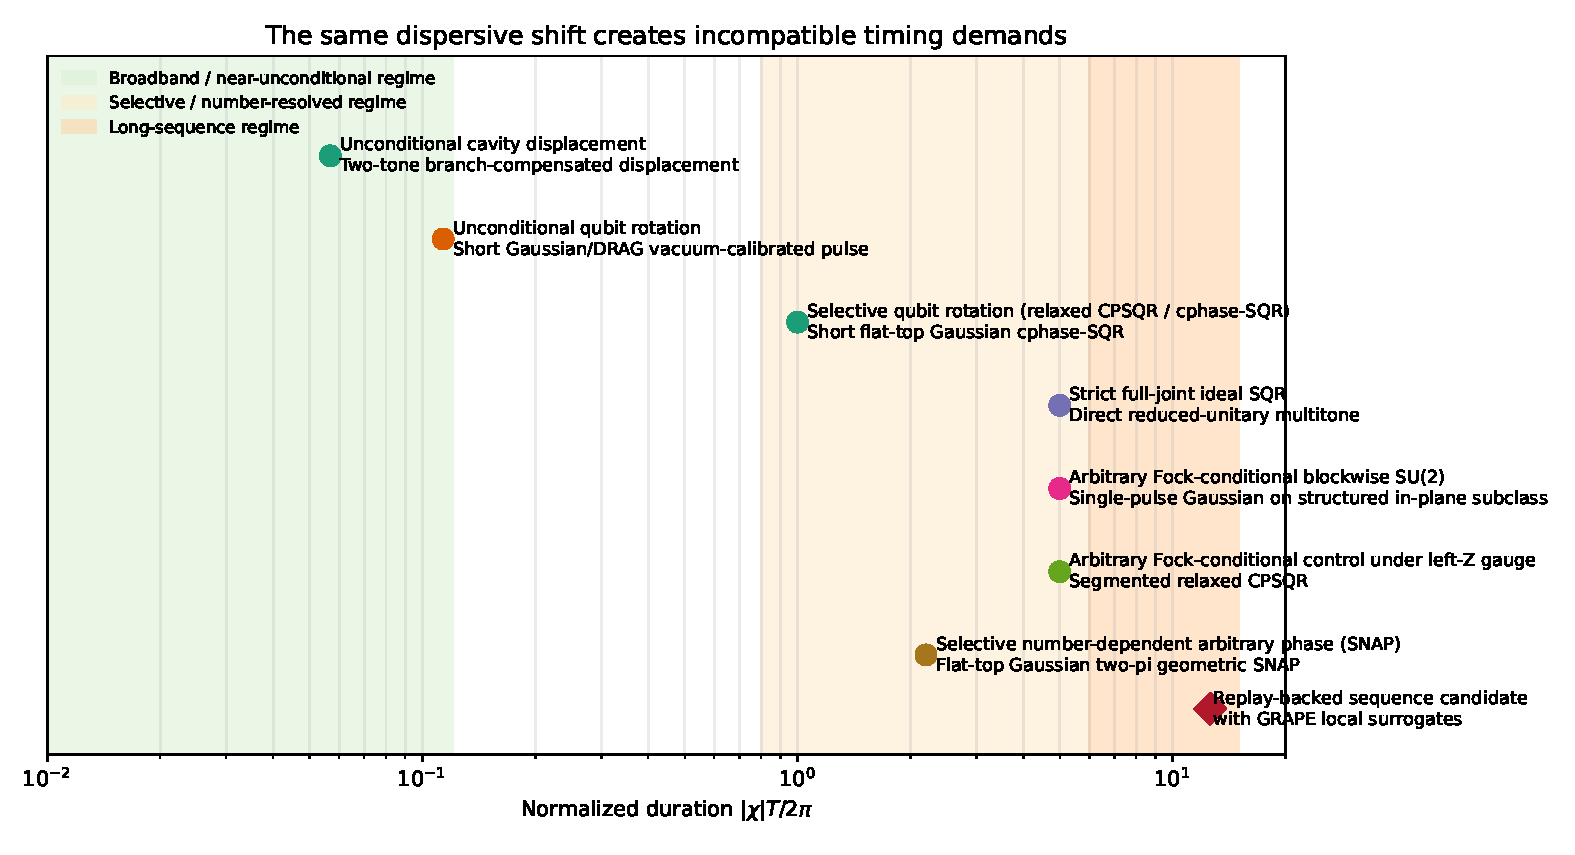
\includegraphics[width=\textwidth]{timescale_hierarchy.pdf}
\caption{Normalized pulse durations for the main primitive families. The broadband near-unconditional regime lies at $|\chi|T/2\pi \ll 1$, while the selective regime begins near $|\chi|T/2\pi \sim 1$. The same dispersive shift that enables number selectivity therefore obstructs naive unconditional operations once the cavity is occupied.}
\label{fig:timescale}
\end{figure}

Figure~\ref{fig:phase_budget} makes the same point in terms of phase accumulation. By the time the pulse duration is long enough to support strict selective control, the conditional qubit branch phase already varies by multiple cycles across low cavity manifolds. Any realistic control design must therefore either cancel, absorb, or explicitly account for that phase structure.

\begin{figure}[H]
\centering
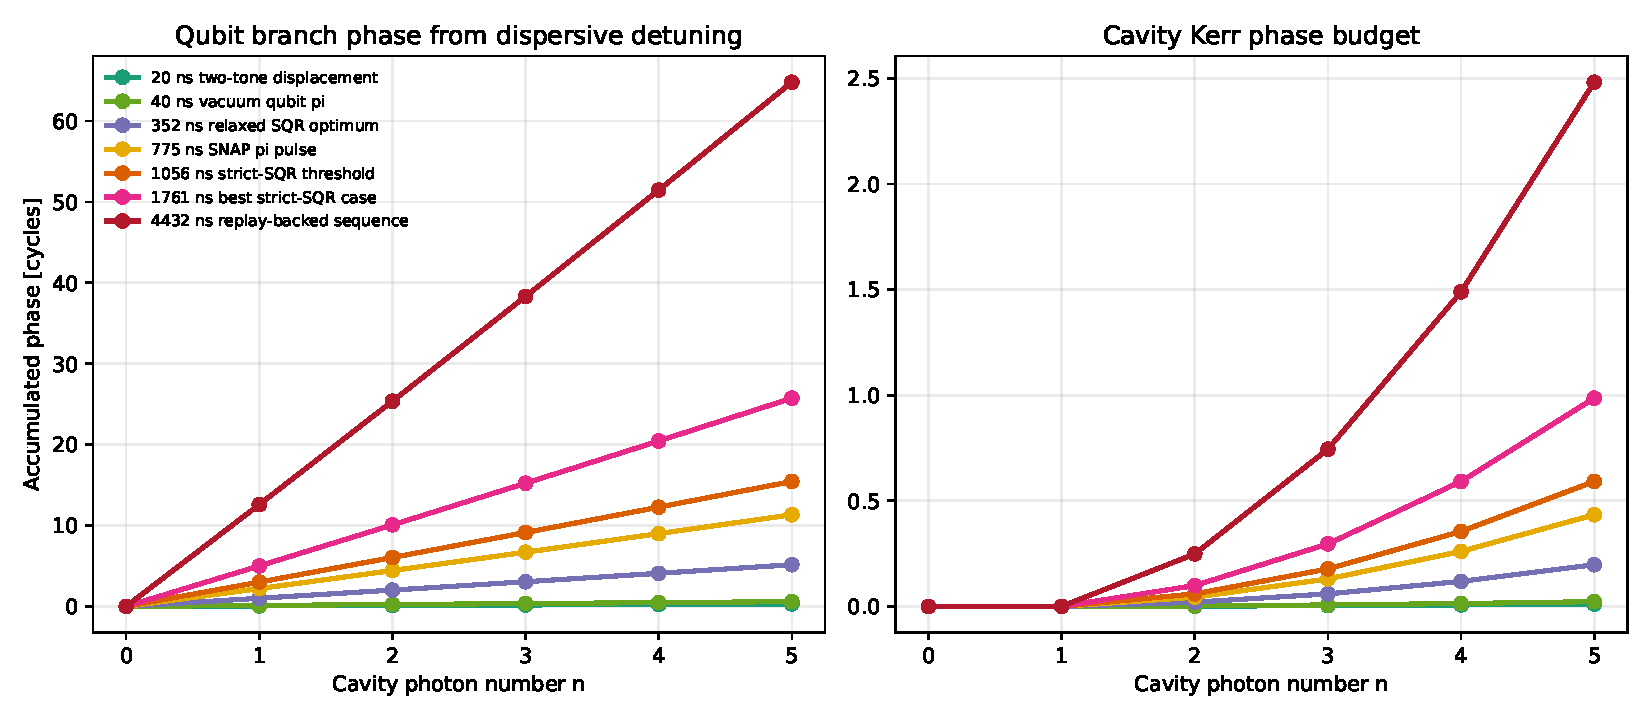
\includegraphics[width=\textwidth]{phase_budget.pdf}
\caption{Representative phase budgets generated from the repository device point. Left: qubit branch phase cycles from the dispersive detuning in Eq.~\eqref{eq:qubit_detuning}. Right: cavity Kerr phase cycles. The main obstruction is already visible without invoking decoherence: once the duration enters the selective regime, manifold-dependent phase accumulation becomes an order-unity effect.}
\label{fig:phase_budget}
\end{figure}

\section{Evidence Synthesis for the Primitive Library}
\label{sec:evidence}

\subsection{Unconditional Cavity Displacement}

The displacement-focused study shows that the ideal primitive
\begin{equation}
U_{\mathrm{disp}} = I_q \otimes D(\alpha)
\end{equation}
is not generically realized by a single resonant cavity pulse once the qubit is allowed to occupy both computational states. The best simple constructive result is a short two-tone branch-compensated pulse at \SI{20}{ns}, corresponding to $|\chi|T/2\pi = 0.057$. On the explicit broad-state benchmark it reaches mean fidelity $0.9857$ and minimum fidelity $0.9242$. The same study also shows that a naive echo built from vacuum-calibrated qubit inversions is not competitive because the inserted inversion pulse inherits its own manifold dependence once the cavity is populated.

The physical interpretation is therefore narrow but useful: unconditional displacement survives only as a \emph{short calibrated multiplex primitive}. The primitive remains available, but not in the naive form suggested by the ideal abstraction.

\subsection{Unconditional Qubit Rotations}

The waveform-level study gives the strongest direct negative result for the ``easy'' qubit primitive. A vacuum-calibrated Gaussian or DRAG $X_\pi$ pulse can be nearly ideal in the vacuum manifold: the reported \SI{40}{ns} pulse reaches fidelity $0.99984$. Yet the same pulse is not unconditional once photons populate the cavity. The same study reports that the Fock-resolved fidelity falls to roughly $0.483$ by the $n=5$ manifold, and that applying the pulse with the cavity in a coherent state of amplitude $|\alpha|=2$ generates about $0.54$ bits of qubit--cavity entanglement.

This is a decisive claim-boundary result. In realistic dispersive cQED, the practical primitive is not a truly unconditional qubit rotation. It is a \emph{spectator-limited short qubit pulse}, whose acceptable cavity-occupation window must be tracked explicitly.

\subsection{Relaxed Selective Qubit Control}

The literature-informed selective-pulse study identifies the strongest practical selective primitive under noise. The best noisy phase-relaxed selective rotation is a short flat-top Gaussian pulse at $|\chi|T/2\pi = 1.0$ with average relaxed fidelity $0.9903$. The corresponding strict logical fidelity is only about $0.892$, which is itself informative: most of the remaining error is conditional phase structure rather than failure to perform the intended selective qubit action.

This is the first major positive result of the synthesis. The physically natural selective primitive is not strict ideal SQR, but a \emph{phase-aware selective rotation} whose residual branch phases are cleaned up later.

\subsection{Strict Full-Joint Ideal SQR}

The strict-SQR feasibility study sharpens the claim boundary further. The strongest direct multitone waveform reaches full-joint strict process fidelity $0.9988$, but only on easier cases with low active dimension and favorable target structure. The same study reports that the direct strict threshold $F_{\mathrm{joint}} \ge 0.99$ is reached at $|\chi|T/2\pi = 3.0$ for the easier regimes, yet it is \emph{not} reached on the harder $\chi+\chi'$ case with three active manifolds, where the best strict joint fidelity saturates near $0.9846$.

Echo changes the story only after the target is relaxed. The best echoed construction reaches essentially unit joint fidelity for the relaxed conditional-phase selective-rotation target, while its strict joint fidelity on the same pulse remains only $0.868$. This proves that manifold-wise qubit success does not certify the full joint operator. The missing resource is not generic transverse control, but the strict inter-manifold phase structure.

\subsection{Arbitrary Fock-Conditional Control}

The arbitrary conditional-control validation study makes the same distinction more sharply. Under a strict blockwise SU(2) criterion, the overall success rate is only $6.8\%$. Under an explicit left-$Z$ gauge relaxation, the success rate rises to $36.8\%$, and the segmented relaxed family reaches relaxed joint-process fidelity $0.99999998$ on a hard random-target slice while the strict joint fidelity on the same pulse is only $0.015$.

This is the strongest evidence that the realistic constructive primitive library is fundamentally phase aware. Once hard target classes are included, a broad positive claim for strict arbitrary blockwise control is not supported. A broad positive claim for phase-relaxed conditional control \emph{is} supported.

\section{Universality Verdict}
\label{sec:verdict}

\subsection{What Fails Literally}

Taken together, the inherited studies rule out the literal version of the ideal primitive claim.

\begin{enumerate}
\item \textbf{Selective qubit rotations are not generically strict ideal operators.} They are strict only on restricted low-dimensional cases and otherwise relax naturally to a phase-aware primitive.
\item \textbf{Unconditional cavity displacement is not a naive one-tone primitive.} It survives only as a short explicitly branch-compensated control.
\item \textbf{Unconditional qubit rotation is not truly unconditional once the cavity is occupied.} It survives only as a short pulse with a bounded spectator window.
\end{enumerate}

Table~\ref{tab:primitive_matrix} summarizes the resulting primitive-level verdicts.

\begin{table}[H]
\centering
\caption{Primitive-level verdicts synthesized from the repository studies.}
\label{tab:primitive_matrix}
\begin{tabular}{p{2.5cm}p{2.8cm}p{1.6cm}p{1.35cm}p{2.7cm}}
\toprule
Primitive & Best structured family & Metric & $|\chi|T/2\pi$ & Verdict \\
\midrule
Unconditional cavity displacement & Two-tone branch-compensated displacement & Broad-state mean fidelity 0.9857 & 0.057 & Approximate success on short calibrated pulses \\
Unconditional qubit rotation & Short Gaussian/DRAG vacuum-calibrated pulse & Vacuum X\_pi fidelity 0.9998 & 0.114 & Only spectator-limited, not truly unconditional \\
Selective qubit rotation (relaxed CPSQR / cphase-SQR) & Short flat-top Gaussian cphase-SQR & Noisy relaxed fidelity 0.9903 & 1.000 & Robust practical primitive \\
Strict full-joint ideal SQR & Direct reduced-unitary multitone & Joint process fidelity 0.9988 & 5.000 & Limited to easy low-window cases \\
Arbitrary Fock-conditional blockwise SU(2) & Single-pulse Gaussian on structured in-plane subclass & Strict joint process fidelity 0.9957 & 5.000 & No general success on hard classes \\
Arbitrary Fock-conditional control under left-Z gauge & Segmented relaxed CPSQR & Relaxed joint process fidelity 1.0000 & 5.000 & Strong positive result under explicit gauge relaxation \\
Selective number-dependent arbitrary phase (SNAP) & Flat-top Gaussian two-pi geometric SNAP & Noisy average state fidelity 0.9377 & 2.200 & Useful but slow cleanup primitive \\
\bottomrule
\end{tabular}
\end{table}

\subsection{What Survives in a Weaker Form}

The realistic constructive library that remains scientifically defensible is:
\begin{enumerate}
\item short branch-compensated displacement rather than naive unconditional displacement;
\item short spectator-limited qubit pulses rather than strictly unconditional qubit rotations;
\item phase-relaxed selective control rather than generic strict SQR;
\item an explicit cleanup layer, such as SNAP or virtual-$Z$ correction, to remove the residual gauge;
\item native dispersive conditional phase when a true entangling primitive is needed at the sequence level.
\end{enumerate}

This is not a cosmetic rephrasing. It is a structural change in the control problem. The universal-control claim survives only after the primitive library is changed from an ``ideal gate'' language to a \emph{phase-accounting} language.

\subsection{Why This Is Not Yet a Fully Demonstrated Non-GRAPE Universal Stack}

The sequence-level runtime study provides the decisive practical constraint. Its best replay-backed hybrid-unitary candidate still relies on GRAPE-derived local surrogates and reaches only process fidelity $0.90269$ in the closed system, with noisy average probe fidelity $0.61448$ at total duration \SI{4.432}{\micro s}. This is not a failure of the native dispersive entangler alone. It is the cumulative consequence of slow local selective layers, replay mismatch, and coherence cost.

The repository therefore supports the following statement and no stronger one: a physically meaningful, structured, and experimentally interpretable \emph{phase-aware} hybrid-control library exists and works well on several low-dimensional primitive tasks, but a fully pulse-backed non-GRAPE universal architecture has not yet been demonstrated.

\section{Conclusion}

The main answer is now unambiguous.

\begin{itemize}
\item The ideal primitive gate set of selective qubit rotations, cavity displacements, and unconditional qubit rotations does not survive literally once $\chi$, $\chi'$, Kerr, and finite-duration phase accumulation are enforced.
\item Unconditional cavity displacement survives only as a short branch-compensated multiplex primitive.
\item Vacuum-calibrated qubit rotations do not remain unconditional in the presence of cavity photons; they become spectator-limited pulses whose safe occupation window must be tracked explicitly.
\item The strongest practical selective primitive is a phase-relaxed selective rotation, not generic strict full-joint ideal SQR.
\item Strict full-joint ideal SQR is achievable only on restricted easy cases, while arbitrary strict blockwise control is not convincingly demonstrated on hard target classes.
\item A phase-aware constructive route does survive: short branch-compensated displacement, short spectator-limited qubit pulses, relaxed selective control, and a later cleanup layer such as SNAP or virtual-$Z$ correction.
\item Even with partial GRAPE assistance, the best current replay-backed sequence-level architecture is still not hardware-ready, so a fully validated non-GRAPE universal stack remains open.
\end{itemize}

In that precise sense, the ideal universal-control claim becomes weaker but more useful. What survives is not a simplistic primitive gate picture, but a realistic design rule for how to build hybrid control around the actual dispersive Hamiltonian.

\section{Limitations and Future Work}

\subsection{Known Limitations}
\begin{itemize}
\item This study is a synthesis of validated repository results plus a first-principles timing and phase analysis; it is not a new large-scale sweep over the entire control landscape.
\item Most inherited strict-control studies are closed-system and use a two-level optimization loop. The main positive and negative claim boundaries should be rechecked under stronger open-system and higher-transmon-level objectives.
\item The sequence-level runtime evidence is strongest for low-dimensional logical windows. Larger encodings may shift the balance further toward native conditional-phase primitives and away from long selective sequences.
\item The present synthesis deliberately avoids turning GRAPE into the conceptual answer. That makes the scientific conclusion cleaner, but it also means the report does not claim a tight ultimate upper bound on what constrained control could achieve.
\end{itemize}

\subsection{Required Follow-Up}
\begin{itemize}
\item \textbf{[P1 | MEDIUM]} Optimize composite families directly against the full strict joint operator, including inter-manifold phase terms in the objective, to determine whether the present strict failure is fundamental or mostly ansatz limited.
\item \textbf{[P1 | MEDIUM]} Replay the strongest strict and relaxed cases with explicit $n_{\mathrm{tr}}=3$, cavity Kerr, and noise in the optimization loop rather than only in post hoc validation.
\item \textbf{[P1 | HIGH]} Build a genuinely pulse-backed phase-aware universal stack using the surviving constructive primitives and test it on at least one nontrivial hybrid target without hiding the local layers inside unconstrained GRAPE.
\item \textbf{[P2 | MEDIUM]} Compare SNAP cleanup against virtual-$Z$ cleanup after the best relaxed selective rotations to determine the lowest-overhead route to strict logical gauge restoration.
\item \textbf{[P2 | MEDIUM]} Extend the same synthesis to cat and binomial encodings, where the balance between branch-compensated displacement, relaxed selective control, and cleanup layers may change.
\end{itemize}

\appendix

\section{Study Composition}

This synthesis consolidates the following validated repository components:
\begin{enumerate}
\item the waveform-level regime study for unconditional displacement and spectator qubit rotations;
\item the literature-informed selective-pulse benchmark for noisy selective rotation and geometric SNAP;
\item the strict ideal-SQR versus relaxed CPSQR feasibility study;
\item the strong-validation study for arbitrary Fock-conditional control;
\item the runtime hybrid-unitary study for sequence-level replay readiness.
\end{enumerate}

Each inherited component remains the source of record for its own underlying simulations. The present report adds only the analytic timescale/phase synthesis, the unified primitive verdict table, and the integrated universality conclusion.

\section{Reproducibility and Saved Artifacts}

The machine-readable outputs created directly by this synthesis study are:
\begin{itemize}
\item a unified summary JSON containing the primitive verdicts, analytic phase budgets, and top-level universality verdict;
\item a machine-readable primitive-verdict artifact;
\item a machine-readable analytic phase-budget artifact;
\item the timing-hierarchy and phase-budget figures in both raster and vector formats;
\item a reproducibility notebook that loads the saved summary by default and includes a commented rerun cell for the synthesis builder.
\end{itemize}

The notebook exposes all tunable parameters in a single early cell, rebuilds all derived paths from those parameters, and defaults to loading saved results rather than rerunning the builder.

\bibliographystyle{unsrtnat}
\bibliography{references}

\end{document}
